\begin{figure}[!t]
{\hspace{-1.3cm}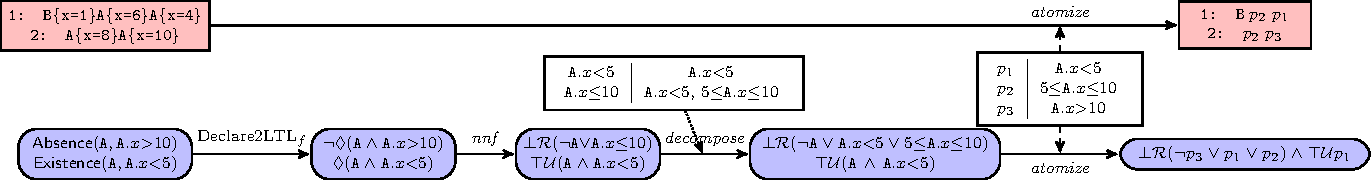
\includegraphics[width=1.3\textwidth]{images/example_1}}

{\hspace{-1.3cm}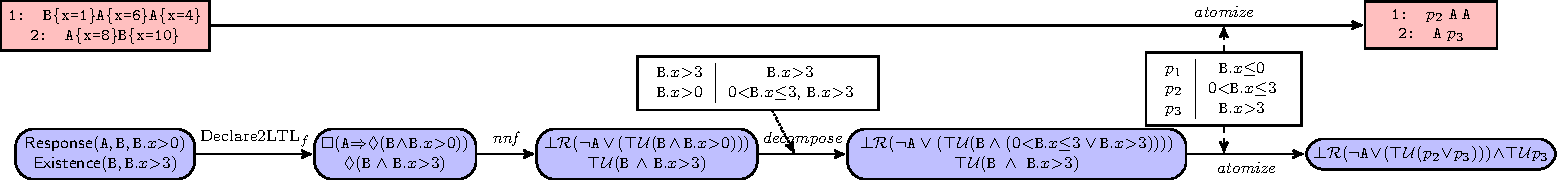
\includegraphics[width=1.3\textwidth]{images/example_2}}

\caption{Two examples (one above, the other below) of input transformation for the $\sigma\tilde{\vDash}\varphi$ Blue boxes represent the Data-Aware Declare model representations, while the red boxes represent the traces' transformation.}\label{fig:twoexamples}
\end{figure}

\section{Data-Aware Declare Trace Alignment Pipeline}\label{sec:dadtap}
We now describe the main contribution of the paper, namely a technique for computing log trace alignments over Declare Data-Aware models. Our approach takes as input \begin{enumerate*}[label=\emph{\alph*})]
	\item a Declare Data-Aware model $\mathcal{M}$ expressed as a set of instantiated templates,
	\item a log trace $\sigma$,
\end{enumerate*} and ranks the outcome of a LTL$_f$ conformance checking $\sigma\tilde{\vDash}\varphi$ accordingly to a data distance function $\mathcal{D}$.

\subsection{Input transformation}
The input transformation for reducing the data-aware alignment problem to the data-agnostic one is presented in Figure~\ref{fig:twoexamples} for two alignment examples. In particular, we first transform the Data-Aware Declare model, for then collecting the required information for providing the trace transformation.

\textbf{Data-Aware Declare Model Processing.} In step 1, we exploit the usual conversion of each single Declare clause into a LTL$_f$ formula, and data-aware predicates are considered as unitary predicates. 

In step 2, we transform each LTL$_f$ formula in negated normal form (\textit{nnf}) and we push the negation within the data-aware predicate: e.g., $\neg(\texttt{A}.x>10)$ is represented as $\texttt{A}.x\leq 10$.

In step 3, we collect the data-aware predicates ``$\texttt{A}.\textit{var}\;\Re\;c$'' from all the model's clauses and group them by $\texttt{A}.\textit{var}$; each of these predicates is \textit{decomposed} into a disjunction maximal non-overlapping data-aware predicates. This task can be efficiently computed via interval trees \cite{inttree}. E.g., predicates $\texttt{B}.x>3$ and $\texttt{B}.x>0$ are first represented as intervals $\interval({3,+\infty})$ and $\interval({0,+\infty})$, and then decomposed into disjoint sub-invervals $\interval({-\infty,0}]$, $\interval[{0,3}]$, and $\interval({3,+\infty})$. 

In step 4, for each event label \texttt{A}, we partition the data space \textit{var}$_1\times\dots\times$\textit{var}$_h$ associated to \texttt{A} by exploiting the disjoint intervals mined in the previous step. Each of such combination will be syntactically represented as a fresh \textit{atom}  proposition $p_i$: this implies that the label \texttt{A} is represented by the disjunction $\bigvee_ip_i$. When the data space associated to the predicates mined for \texttt{A} has only one property,  the atoms corresponds to the ones mined in the previous step. E.g., \texttt{A} in the first example from \ref{fig:twoexamples} is equivalent to $p_1\vee p_2\vee p_3$, and $\texttt{A}.\textit{x}<5$ is rewritten as $p_1$; given that such atoms represent disjoint intervals, then $\texttt{A}\wedge p_1\equiv p_1$. Similarly, $\neg \texttt{A}\vee \texttt{A}.\textit{x}<5\vee 5\leq\texttt{A}.\textit{x}\leq 10$ can be immediately rewritten as $\neg(p_1\vee p_2\vee p_3)\vee p_1\vee p_2$, which is equivalent to $\neg p_3\vee p_1\vee p_2$. Last, each LTL$_f$ representation of a Data-Aware Declare clause is represented into one single LTL$_f$ formula by conjunction and simplification.

\textbf{Data-Aware Log Trace Processing.} Given the atomization in Step 4, we process each data-enriched event within the trace as follows: if the event label is never associated with a data predicate, then we just discard the data information; otherwise, we replace each event with the single corresponding atom satisfying the associated semantics. Please observe that, by previous construction, each event can be represented by just one possible propositional atom, as the previous construction guarantees a partitioning (thus non-overlapping) representation of the data space.

\subsection{Output transformation} \texttt{\color{red}[TODO]}